%!TEX root = ..our_P/introduction.tex
\section{Introduction}
\label{sec:introduction}
There are a variety of software applications and services (online games, social networks, search engines, etc.) in the Internet companies, which are monitored with some KPI data (key performance indicator, \EG, CPU utilization, number of queries per second, response delay). These KPIs are usually displayed in the time series format, also known as KPI streams. Operation engineers constantly monitor and detect anomalies for KPI streams to provide reliable services.
Anomalies in KPI streams always manifest as spikes or sudden drops, indicating potential failures of Internet services~\cite{chen2013provider,liu2015opprentice,zhang2015rapid} (server failures, network overload, external attacks, etc.).
%Anomaly detection encounters associated with
Moreover, new products and services are constantly produced, %are launched endlessly plenty of
resulting in endless KPI streams,
which emerges a big challenge for anomaly detection.

% \textcolor{red}{On the other hand, %with the popularity of DevOps and micro-service,
% software upgrades more and more frequent~\cite{zhang2016funnel}, resulting in the pattern changes of existing KPI streams, which makes the previous anomaly detection algorithms/parameters outdated.}
%There remains a scenario that when a large number of KPI streams emerge frequently and continuously, operators need to deploy accurate anomaly detection models as soon as possible (\EG, within 3 weeks at most),
%which aims to avoid %that Internet-based services suffer
%suffering from false and missing alarms
%(due to low precision) and/or missed alarms (because of low recall),
%and in turn impact on user experience and revenue.

Although a great quantity of KPI anomaly detection algorithms have been proposed~\cite{chen2013provider,liu2015opprentice, knorn2008adaptive, pincombe2005anomaly, yan2012argus, lu2009network, egads, ding2013anomaly} over the years,
which are mainly divided into supervised learning and unsupervised learning methods, none of them are feasible to deal with the above scenario well unfortunately:
\begin{itemize}
  \item  
  Supervised learning based methods\cite{egads, liu2015opprentice} require manually labeling anomalies for each KPI stream in the training dataset, while the workload of labeling is very large and often unrealistic in practice.
  \item 
  Unsupervised learning based methods are usually unsatisfactory with a low effectiveness and accuracy~\cite{ding2013anomaly}, as they are trained without the domain knowledge of operators.
%   \textcolor{red}{or require large amounts of training data~\cite{xu2018unsupervised}. At present, with the development of Internet industries, there are lots of KPI streams with new shapes constantly emerging. Because unsupervised learning lacks the domain knowledge of people, learning different KPI shapes is more difficult.}
\end{itemize}

The above two categories of methods are limited, and the current hot idea is semi-supervised learning. For example, ADS~\cite{ADSarticle} enables the rapid deployment of anomaly detection models (say at most 3 weeks) for a large number of emerging KPI streams, without manual algorithm selection, parameter tuning, or labeling for newly emerging KPI streams. %However, 
%Despite %semi-supervised learning based methods
%they perform well, 
They have achieved good performance using the time series segments with high-quality ground truth, i.e., all samples in specific time series segments are required to be carefully labeled (normal or anomalous). Obtaining such labeled data raises another great challenge, because operators need to examine the %part of a
KPI streams back and forth and such a stressful task usually leads in low enthusiasm. 
%This paper mainly focuses on the PU learning.

% \vspace{-3 mm}
\begin{figure}
  \begin{minipage}[h]{1.0\linewidth}
  \centering
  \setlength{\abovecaptionskip}{3.cm}
  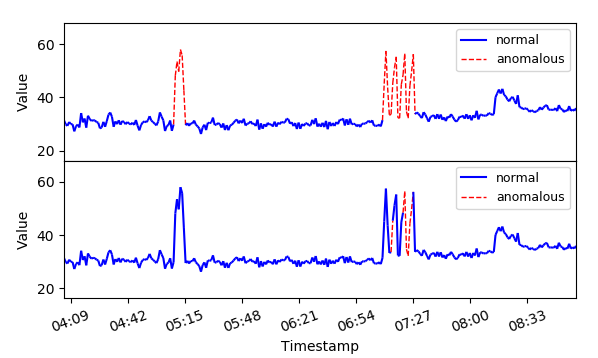
\includegraphics[width=0.9\textwidth]{ADS_Journal/PU figures/Figure_1.png}\\
  \end{minipage}
  \caption{The requirement comparison between Semi-supervised algorithm (upper one) and PU learning algorithm (lower one) for manual labels.}
  \label{fig:comparison_labels}
%   \vspace{-3 mm}
\end{figure}

\begin{figure*}
  \centering
  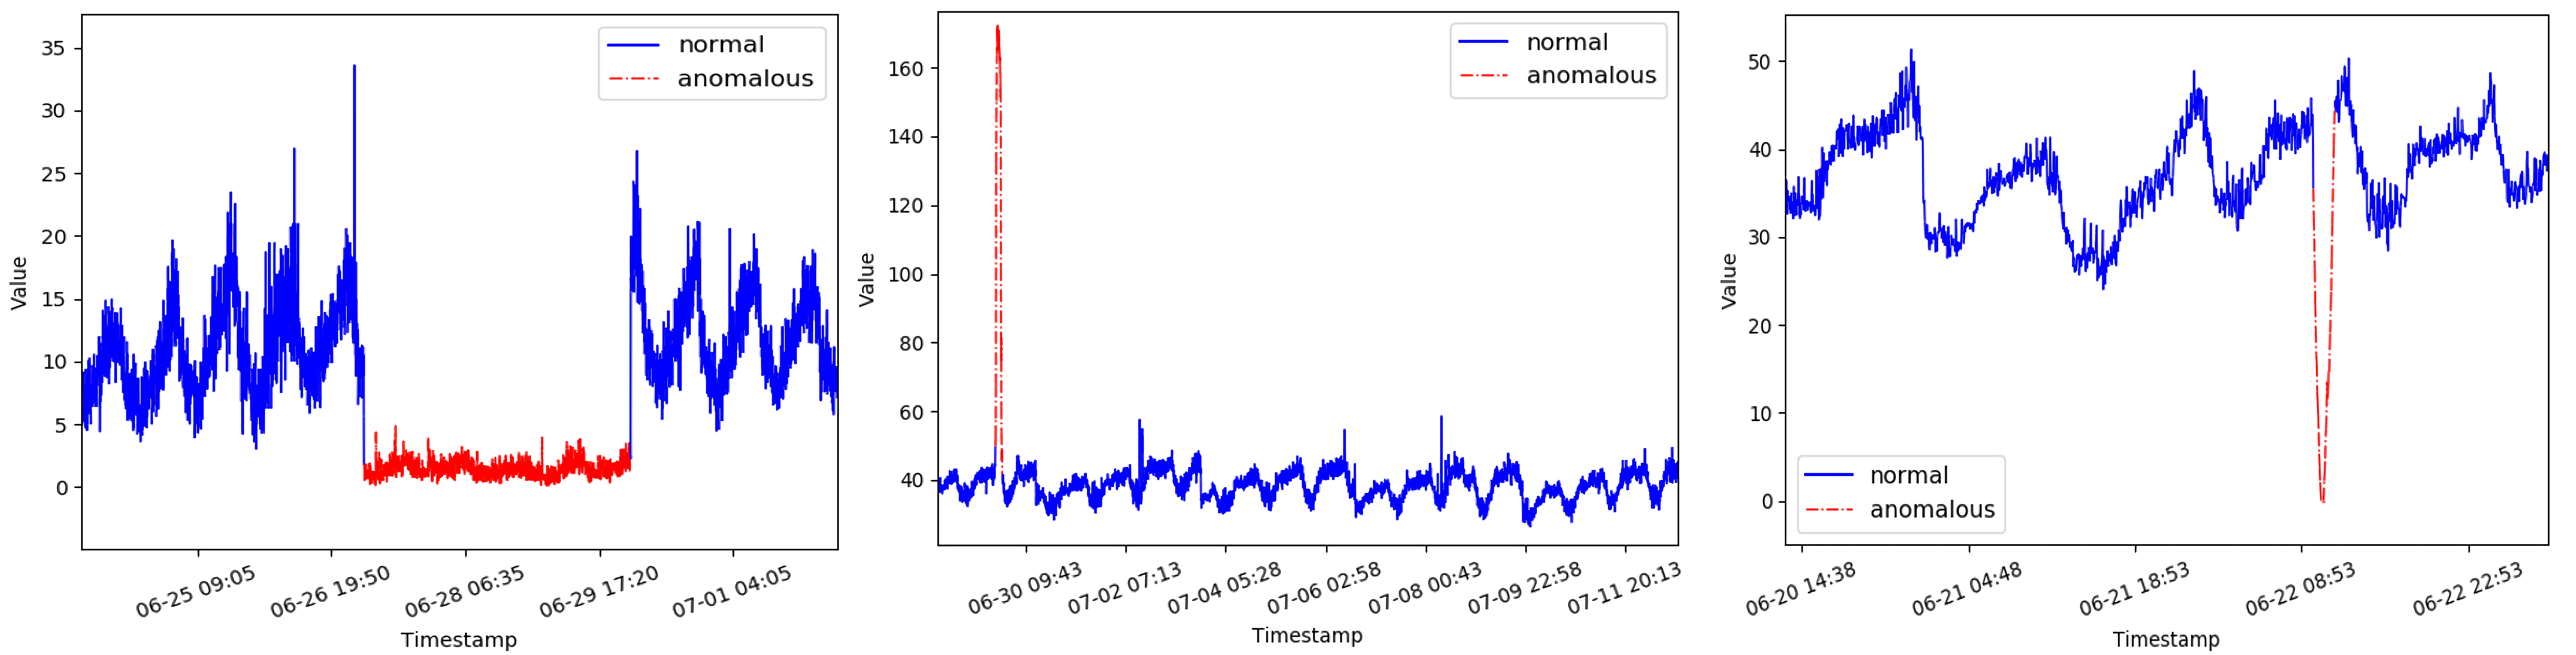
\includegraphics[width=0.9\textwidth]{ADS_Journal/PU figures/fake kpi.png}\\
  \caption{Examples of anomalies in KPI streams. The red parts in the KPI stream denote anomalous points.}
  \label{fig:KPI_anomaly}
%   \vspace{-3 mm}
\end{figure*}

To solve these two challenges, the significant label efforts for large-scale time series, now PU learning has been proposed.
For a specific time series segment, it only needs to label partial anomalous samples carefully, %any few abnormalities
%and performs better than the semi-supervised learning based methods.
%Operators only need to label %several
%partial anomalous samples that workload of them can be reduced greatly and their work enthusiasm will improve
leading to less workload and greater enthusiasm for operators.
Figure~\ref{fig:comparison_labels} shows an example of a time series fragment. The upper and lower subgraphs show the abnormalities that need to be manually labeled for the semi-supervised algorithm and PU learning algorithm, respectively.
%Besides the label efforts, there %face two other challenges
Follow the idea of PU learning, there still mainly faces two challenges:
\begin{itemize}
\item Firstly, most anomaly detection algorithms assume that each KPI needs to be trained in a separate model. Anomaly detection for large-scale time series is very challenging due to the heavy overhead of model selection, parameter tuning, model training, or exception labeling. However, one model for all KPIs often suffers inaccurate prediction, due to the variety of KPI features.
\item Secondly,
the performance of PU learning methods is limited due to the inaccuracy of labels during its iteration, and naturally active learning is proposed to solve this.
%we hope to use the idea of active learning to further improve the performance of PU learning.
%While for time series anomaly detection algorithms,
However, the current active learning methods mainly label the classification boundaries samples~\cite{activelearning2015},~\cite{6747346}, causing some normal samples are misclassified as anomalous with high similarity. 
%into anomalous class.
%Due to the extreme similarity 
%among normal samples, this will cause more normal samples to be incorrectly labeled as anomalous.
\end{itemize}

%In practice, many groups of KPI streams are similar because of their implicit association as well as similarities, therefore we usually use similar anomaly detection algorithms and parameters for each group. Clustering methods can be used to cluster the KPI streams into some clusters according to their similarities. The number of clusters is largely determined by the nature of the service (\EG, shopping, gaming, social network) and the type of KPIs (\EG, number of queries, CPU usage, memory usage). Thus for a given service, the number of clusters can be orders of magnitude smaller than the number of KPI streams, and there is a good chance that a newly emerging KPI stream falls into one of the existing clusters resulted from historical KPI streams.

To solve the above challenges, we propose \name{}, the first framework applying the PU learning algorithm to time series anomaly detection,
which consists of three major components:
(1) Pre-clustering. Clustering the KPI streams into some clusters according to their shape similarities. The number of clusters is much smaller than the number of KPI streams which greatly reduces the amount of data we have to process. Moreover, for a newly emerging KPI stream, it can be assigned into the existed clusters based on its similarities with the clusters. 
(2) PU learning. Utilize PU learning to generate labeled samples with high reliability. PU learning method aims to build a binary classifier from only positive (anomalous) and unlabeled data of cluster centroids. 
% Through PU learning, we can train a final model with less labeled data which eases the difficulty of labeling. 
It allows our initial data to have very few labels, which reduces the difficulty of manual labeling. However, commonly used PU learning methods always mistakenly label some negative samples as positive which leads to a bad performance. Therefore, we adopt active learning to check reliable positive samples to improve the performance of PU learning.
(3) Semi-supervised method. When having labeled enough label, a semi-supervised method is used to train a final anomaly detection model for each cluster centroid.

%Utilizing the above analysis, the process overview of \name{} is as follows:
%\begin{itemize}
%  \item  
%  Cluster all existing/historical KPI streams into clusters.
%  \item 
%  Randomly label the anomalies of all cluster centroids manually and extract features of them.
%  \item
%  Exploit cluster centroids as the training set and use PU learning with active learning to train a model for each centroid.
%  \item
%  When emerging a new KPI stream, assign it into one of the existing models to detect anomalous samples.
%\end{itemize}

%In conclusion, \name{} can avoid algorithm selection and parameter tuning. There are only part of anomalous samples in the historical/existing data set at first, so we need to select credible normal samples from unlabeled data. To make the selection more reliable, \name{} uses active learning algorithm~\cite{activelearning2015} which allows the operators to decide whether to manually label or not when facing with samples likely to be anomalous. When enough data is labeled, a semi-supervised method is used to train a final detection model.
%Through experiments, we show that the best F-score achieved by \name{} is over 0.83 on 80 new KPI streams, almost as the same as a state-of-art supervised approach ~\cite{liu2015opprentice}. In addition, \name{} greatly outperforming a state-of-art unsupervised approach ~\cite{xu2018unsupervised}, and better than a semi-supervised learning method ~\cite{ADSarticle}.

The contributions of this paper are summarized as follows:
\begin{itemize}
  \item 
  %Due to implicit association and similarity, the basic shapes of many KPIs are similar.
  We propose to 
  %first
  exploit pre-clustering to process the initial KPI data set. %Subsequent only need to
  Applying an anomaly detection model for each cluster with only labeling the cluster centroid reduces the labeling efforts. 
  %and improves the accuracy of prediction.
  \item  
  It is the first time to apply PU learning to solve the problem of time series anomaly detection. Through PU learning, the operators only need to label a few anomalies randomly. Compared with semi-supervised or supervised learning based methods, it greatly reduces the difficulty of manual labeling.
  \item
  We provide an active learning method using a novel labeling strategy to improve the performance of PU learning. During the process of PU learning, it selects samples that may be positive to label instead of samples that are close to the classification boundary as in many traditional methods. By checking those samples most likely to be positive, we can train a final model with more precise samples to achieve better performance. A large number of experiments have shown that our strategy can improve the average F-score by 8.7\% compared to the other selection strategy. 
  
  % The active learning algorithm applied in this paper is not to label the classification edge samples, but to the samples that may be P. Thus, anomalous samples are avoided from being misclassified into normal samples as far as possible, and the labeling result is more accurate. 
\end{itemize}

The rest of this paper is organized as follows. In Section~\ref{sec:Background}, we introduce the background of our work. The framework of \name{} is introduced in Section~\ref{sec:algorithm}. We report the experimental results of evaluating~\name{} in Section~\ref{sec:evaluation}. Finally, we give a conclusion of this paper in Section~\ref{sec:conclusion}.